%%%%%%%%%%%%%%%%%%%%%%%%% file draft4_2.tex %%%%%%%%%%%%%%%%%%%%%%%%%%%%%%%
%	                                                                   %
% Based on the  template file for The European Physical Journal C          %
%                                                                          %
%                                                                          %
%                                                                          %
%                                                                          % 
%%%%%%%%%%%%%%%%%%%%%%%%% Springer-Verlag %%%%%%%%%%%%%%%%%%%%%%%%%%%%%%%%%%

\documentclass[epj,nopacs]{svjour}
\usepackage{graphics}
\usepackage{epsfig}
\usepackage{latexsym}
\usepackage{amssymb}
\usepackage[utf8]{inputenc}
\usepackage{../../assets/uniinput}

\usepackage{siunitx}
\usepackage[justification=raggedright,singlelinecheck=false]{caption}
\sisetup{
	seperr		=	true,
	trapambigerr	=	true,
	openerr		=	(,
	closeerr	=	),
	expproduct	=	cdot,
	padnumber	=	both,
	stickyper	=	true,
	per		=	slash,
	trapambigfrac	=	true,
	repeatunits	=	false,
	openfrac	=	(,
	closefrac	=	),
	prefixsymbolic 	=	true,
	prefixproduct	=	cdot,
	decimalsymbol	=	.,
        tabnumalign     =       left,
        tabtextalign    =       left
}

\newcommand{\spar}{{\stackrel{\rightarrow}{\Rightarrow}}}
\newcommand{\sant}{{\stackrel{\rightarrow}{\Leftarrow}}}
\newcommand{\sperpa}{{\rightarrow\Uparrow}}
\newcommand{\sperpb}{{\rightarrow\Downarrow}}
\begin{document}
\hugehead

\newcommand{\dd}[1]{\mathrm{d}#1\,} % declare dx operator, usage: \dd{x} for dx
\newcommand{\lref}[1]{listing (\ref{lst:#1})} % refer to a listing, usage:\lref{label} for Listing (...)
\newcommand{\fref}[1]{fig. (\ref{fig:#1})} % refer to a figure, usage:\lref{label} for Abb. (...)
\newcommand{\tref}[1]{tab. (\ref{tab:#1})} % refer to a table, usage:tlref{label} for Tab. (...)
\newcommand{\eref}[1]{eq. (\ref{eqn:#1})} % refer to a equation, usage:\eref{label} for Gl. (...)

\title{Z-Resonance at LEP}
\titlerunning{Z-Resonance at LEP}
\authorrunning{Thomas Murach, Robert Riemann}
\author{{\bf Draft Version 1.1}\\
\medskip \\
Thomas Murach,$^{1}$
Robert Riemann$^{1}$
} 
\institute{$^1$Department of Physics, Humboldt University of Berlin, Germany\\}  
\date{Received: \today / Revised version:}
\abstract{
We had a lot of fun measuring the lifetime and the mass of the Z boson! These quantities 
are important to answer the question of life, universe and everything.
Another nice thing we could access was the number of the lepton families, which we 
were especially happy about...  
}
\maketitle

%%%%%%%%%%%%%%%%%%%%%%%%%%%%%%%%%%%%%%%%%%%%%%%%%%%%%%%%%%%%%%%%%%%%%%%%%%%%%%
\vspace*{-1.5cm}
\section{ Introduction}
\baselineskip=0.38cm
\vspace*{1.cm}

The standard model of elementary particles describes interactions of particles
by four fundamental forces. One of them is the electroweak force. It`s gauge
bosons, which mediate the force between the two interacting particles, are the
photon as well as the W$^{\pm}$- and the Z$^0$-boson. At the
electron-positron-collider LEP at CERN the Z$^0$ has been seen for the first
time, which was possible because of the sufficient center of mass energy of this
collider experiment.

We were able to evaluate it`s mass $M_Z$ and it`s lifetime τ. The leptonic and
the hadronic decay widths $Γ_l$ and $Γ_h$ could be investigated as well. Finally
the number of quark and lepton families $N_C$ and the weak mixing angle, also
called Weinstein angle, $\Theta_W$ can be measured. This angle describes the
ratio of the electric and the weak coupling constants α and α$_w$.

\section{ Experiment}

LEP was designed to be able to deliver center of mass energies $\sqrt{s}$ from
some 89 up to \SI{209}{\giga\electronvolt}. This is enough to produce Z-bosons,
which should have a mass of about \SI{91}{\giga\electronvolt}, as it was
predicted by the standard model. Therefore the Z$^0$-particle was supposed to be
produced at LEP. It can decay in various ways, but always into pairs of one
fermion and one antifermion. One of these possibilities is the decay via two
different quarks (Z$^0→q\overline{q'}$), another one could be the decay via two
charged leptons like Z$^0→ μ^+μ^-$. The first one of the mentioned decays can be
seen as two jets which can be measured in hadronic calorimeters. The leptonic
decay is measured due to registration of leptons in electromagnetic
calorimeters. All of these layers have an almost cylindrical shape in order to
cover as much of the solid angle as possible. This is also the reason for the
installation of the endcaps.

The detector for all of these particles is LEP. Its structure can be seen
in \fref{aufbau}.
\begin{figure}[htb]
 \centering
 \includegraphics[page=5,viewport=286 620 508 765,clip,%
  width=\columnwidth,keepaspectratio]{../../Z0/docs/Z0ResFprakt}
 \caption{Design of the L3 detector\cite{script}}
 \label{fig:aufbau}
\end{figure}
There are layers of components with different purposes, starting from the
interaction point, these are the tracking chamber, the electromagnetic calorimeter,
the hadronic calorimeter and finally the muon chamber.

In our case the hadronic calorimeter and the muon chamber are the most
important parts. The hadronic calorimeter consists of alternating layers of
uranium plates and wire chambers. The muon chamber is built up of drift
chambers. It detects the high energy muons, which have passed the detector
without a significant loss of energy, because these are the only particles that
are able to reach there. Further information about the detector design can
be found in \cite{script}.

\section{ Data analysis}

For a detailed analysis of the mentioned processes it is important to be able
to distinguish between muonic and hadronic decays. We did some Monte Carlo
studies to figure out how these two processes look like. This gave us the
possibility to apply cuts on the measured distributions. In this paper we are
already able to show the results of measurements at center of mass energies of
89.48, 91.33 and \SI{93.02}{\giga\electronvolt}.

\subsection{ Event selection}
Muons barely interact with any matter, therefore there are only very few
entries in the calorimeter along the track of the muon. This has an immense
discriminating power, because jets ...

\subsection{Extraction of the cross section}

Example of an equation:

\begin{equation}
\label{a1vm}
A_{1}^{} = \frac{A^{}_{||}}{D^{}}  - \eta \sqrt{R^{}}\ . \\
\end{equation}


\subsection{Background subtraction}

\begin{figure}[ht]
\vspace*{-0.2cm}
%\resizebox{0.5\textwidth}{0.35\textwidth}{\includegraphics{./r_06m.eps}}
\caption{\baselineskip=0.38cm Example of a picture}
\label{fig:1}   
\end{figure} 
...


\begin{table}[h]
\begin{center}
\begin{tabular}{|l|l|l|}
\hline
\multicolumn{1}{|c|}{}& proton & deuteron\\
\hline
\multicolumn{3}{|c|}{Exclusive electroproduction}\\
\hline
$A^\rho_1$       & 0.23 $\pm$ 0.13$\pm$0.01 & -0.040 $\pm$ 0.076$\pm$0.003\\ 
$A^\phi_1$       & 0.20$\pm$0.45$\pm$0.01  & 0.17$\pm$0.27$\pm$0.01\\
$N^\rho$         &1774                   & 6505\\
$N^\phi$         & 219                   & 618 \\
\hline
\multicolumn{3}{|c|}{Electroproduction by quasi-real photons}\\
\hline
$A^\rho_1$  & 0.0057 $\pm$ 0.0093$\pm$0.0004  & -0.0039 $\pm$ 0.0029$\pm$0.0003\\ 
$A^\phi_1$  & 0.052 $\pm$ 0.084$\pm$0.003  & 0.018 $\pm$ 0.028$\pm$0.001\\
$N^\rho$    & $423\times10^{3}$ & $4013\times10^{3}$\\
$N^\phi$ & $7.6\times10^{3}$ &  $57\times10^{3}$ \\
\hline
\end{tabular}
\vspace*{0.3cm}
\caption{\baselineskip=0.38cm Example of a table}
\label{tab_asy}
\end{center}
\vspace*{-0.5cm}
\end{table}


\section{ Summary}

\begin{thebibliography}{}
\baselineskip=0.38cm
\bibitem{z1} T. H. Bauer et al., Rev. Mod. Phys. \textbf{50} No 2 (1978) 261  
\bibitem{z2}D. Schildknecht et al., Phys. Lett. \textbf{B 449} (1999) 328
\bibitem{z3}A. Donnachie, P. V. Landshoff, Phys. Lett. \textbf{B 478} (2000) 146

\end{thebibliography}

\begin{figure}[htb]
 \centering
 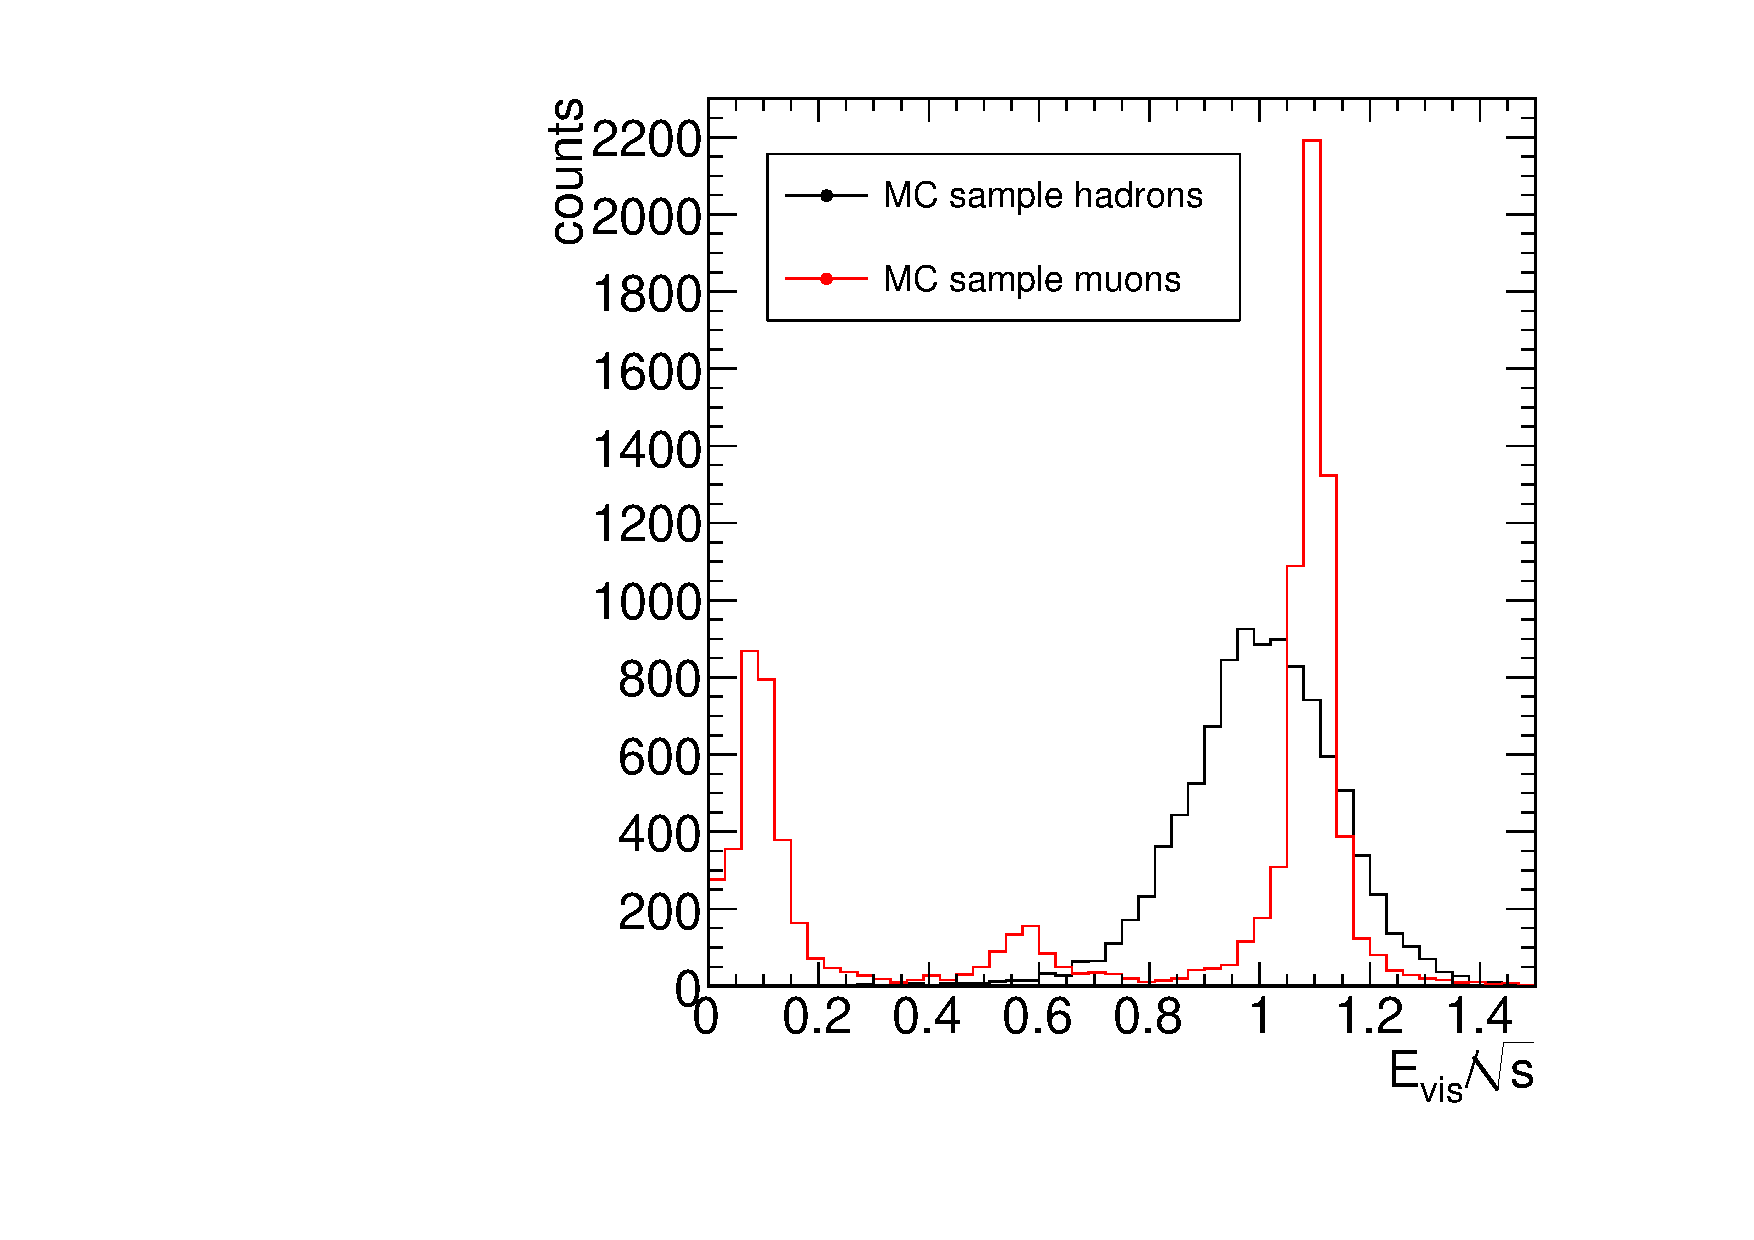
\includegraphics[width=1\columnwidth,keepaspectratio]{E_vis}
 \caption{Distribution of visible energie}
 \label{fig:e_vis}
\end{figure}

\begin{figure}[htb]
 \centering
 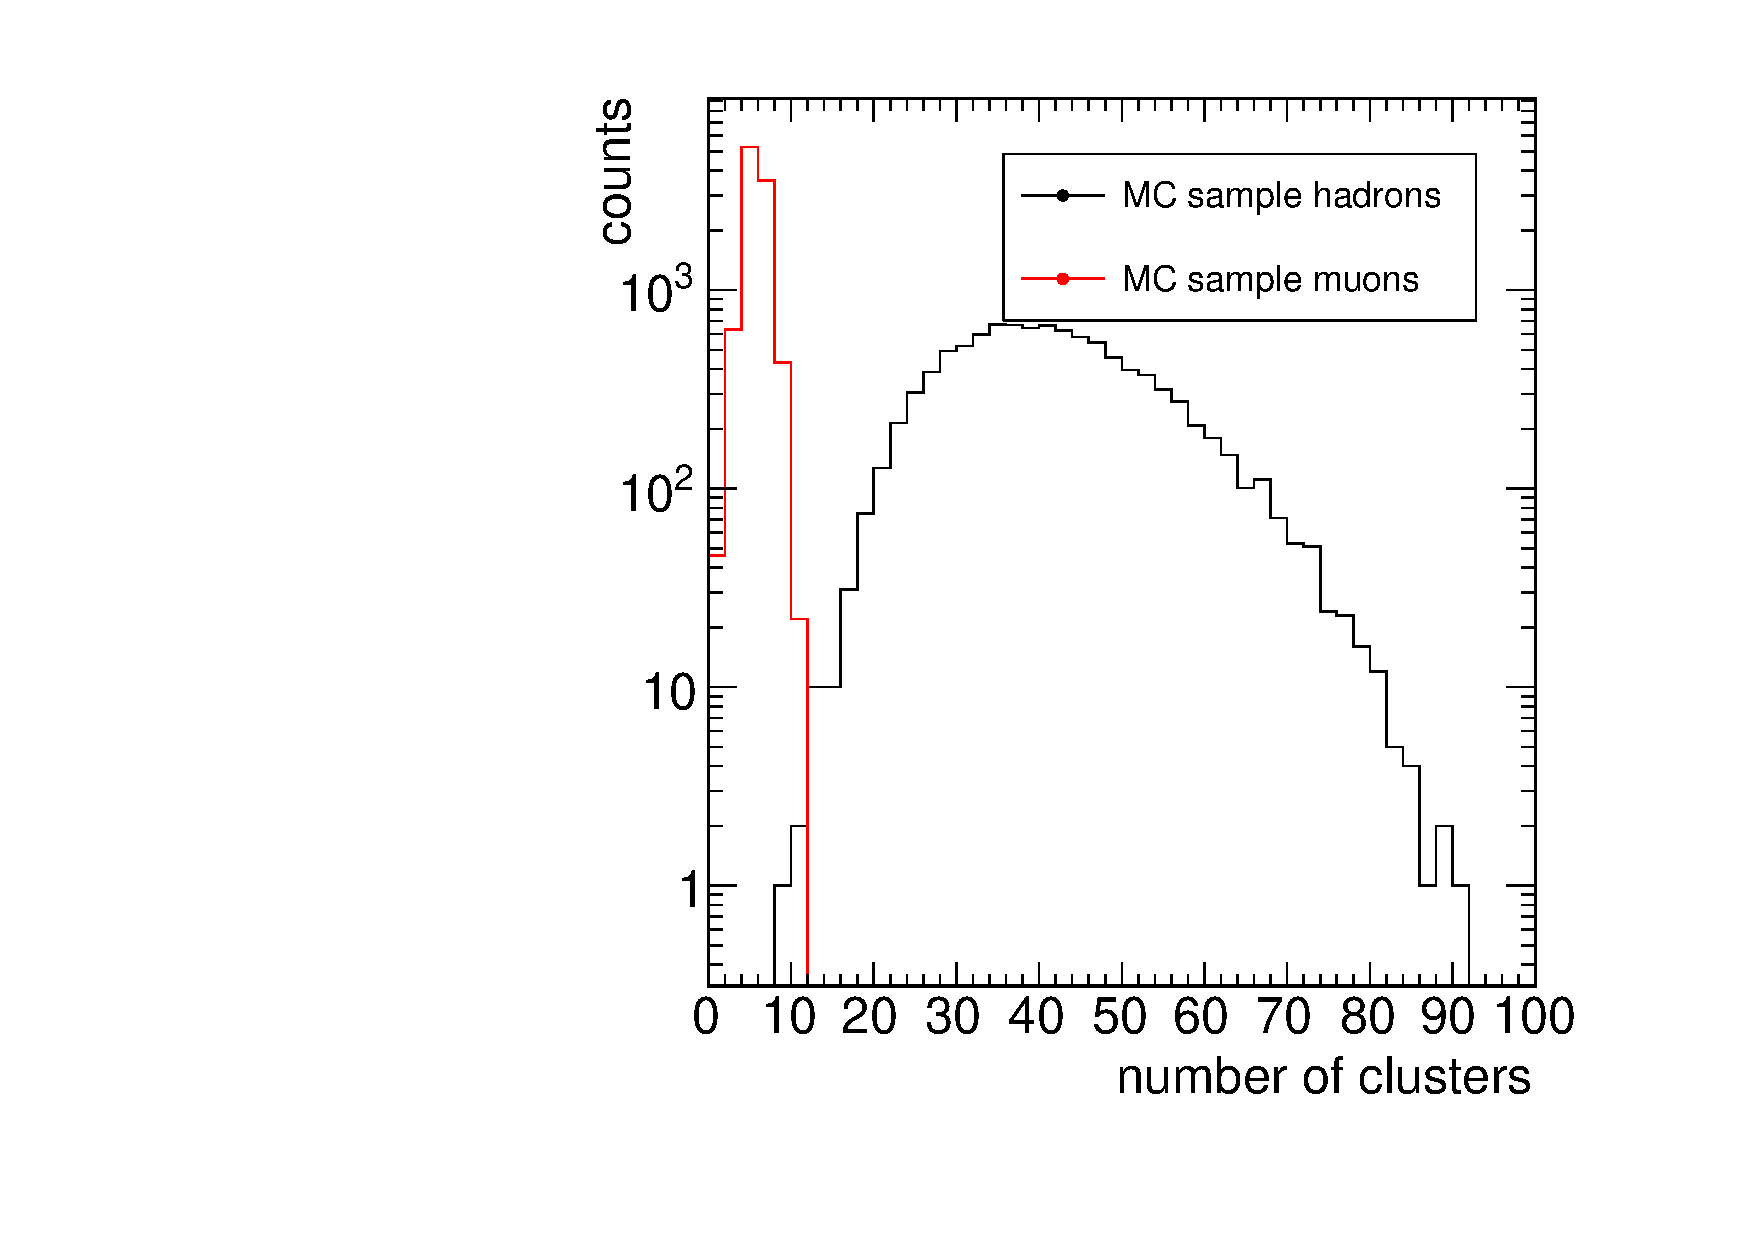
\includegraphics[width=1\columnwidth,keepaspectratio]{N_Cluster}
 \caption{Distribution of entries in the calorimetre}
 \label{fig:n_cluster}
\end{figure}

\begin{figure}[htb]
 \centering
 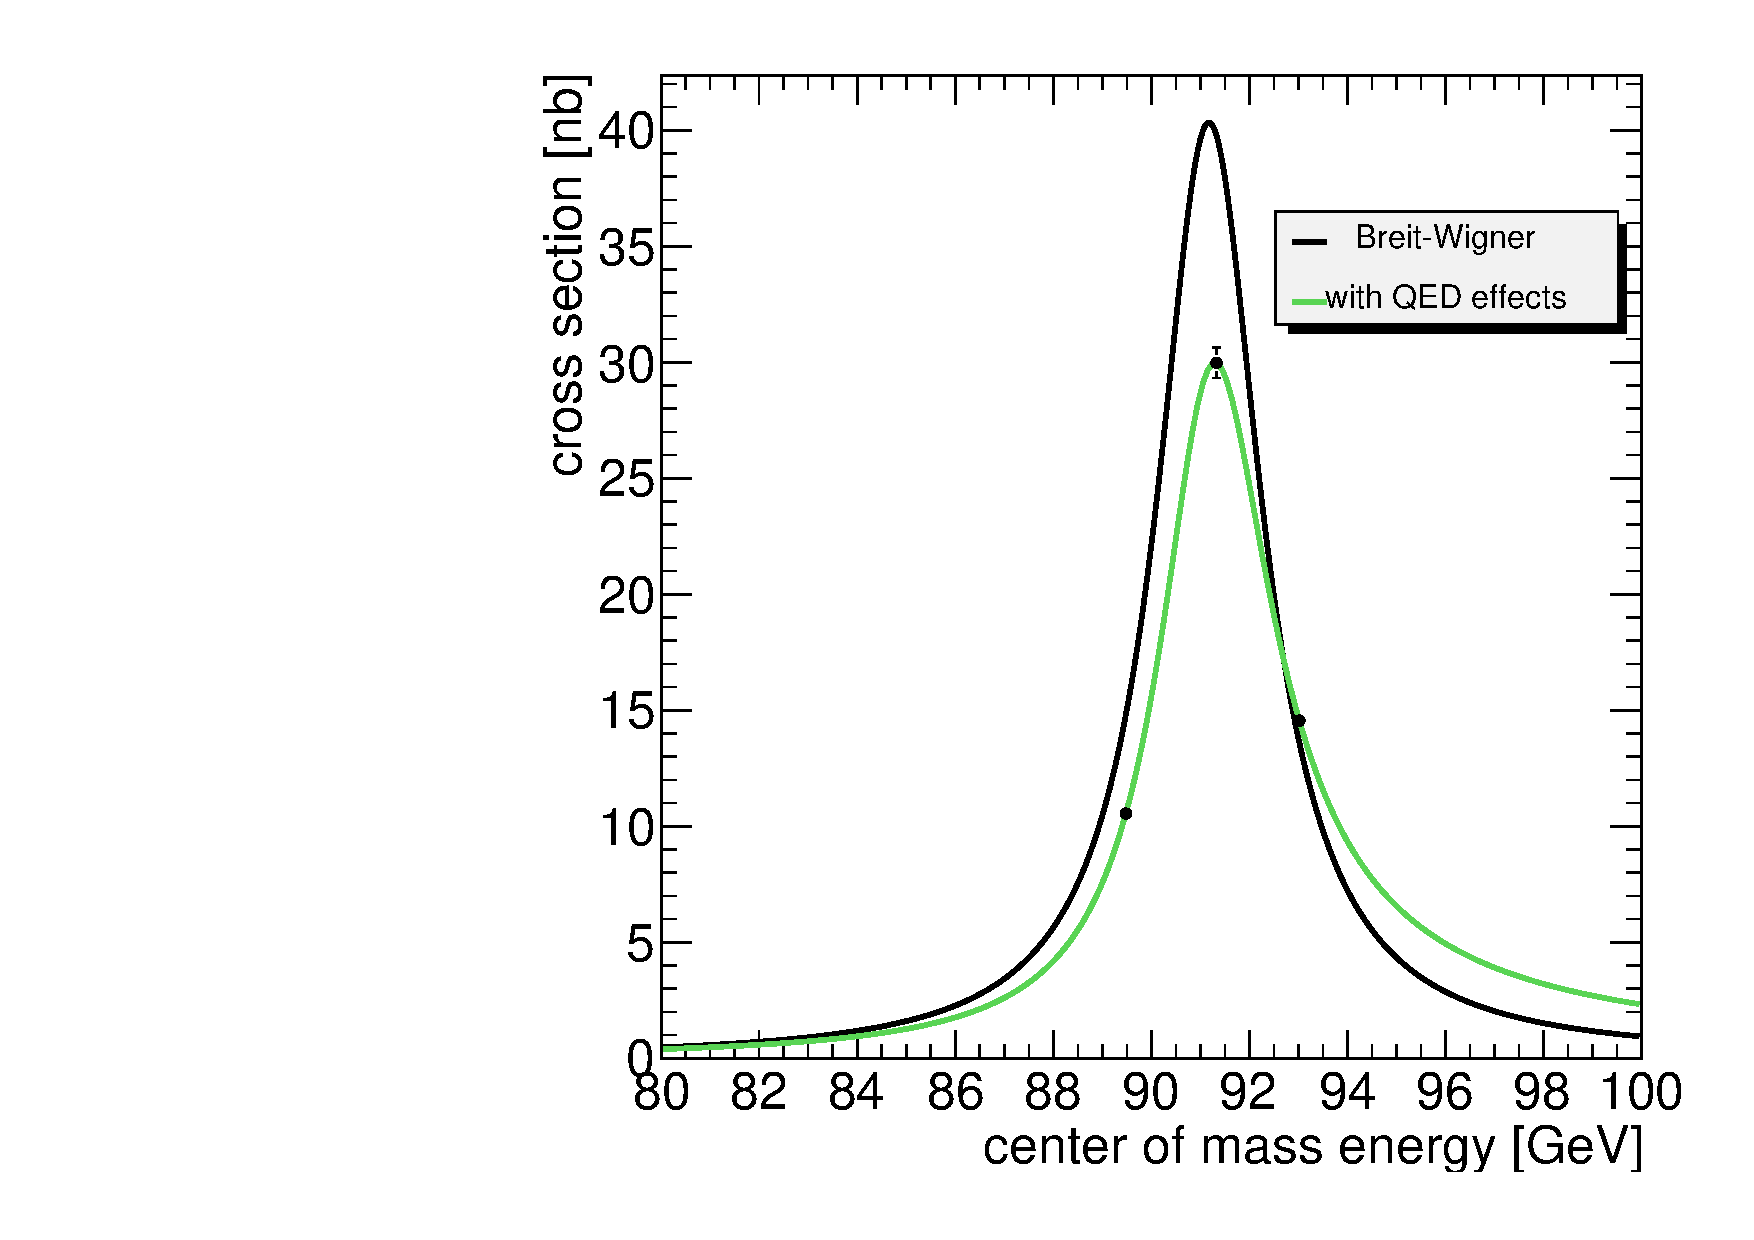
\includegraphics[width=1\columnwidth,keepaspectratio]{finalhad_fit}
 \caption{Breit-Wigner-Fit hadrons}
 \label{fig:e_vis}
\end{figure}

\begin{figure}[htb]
 \centering
 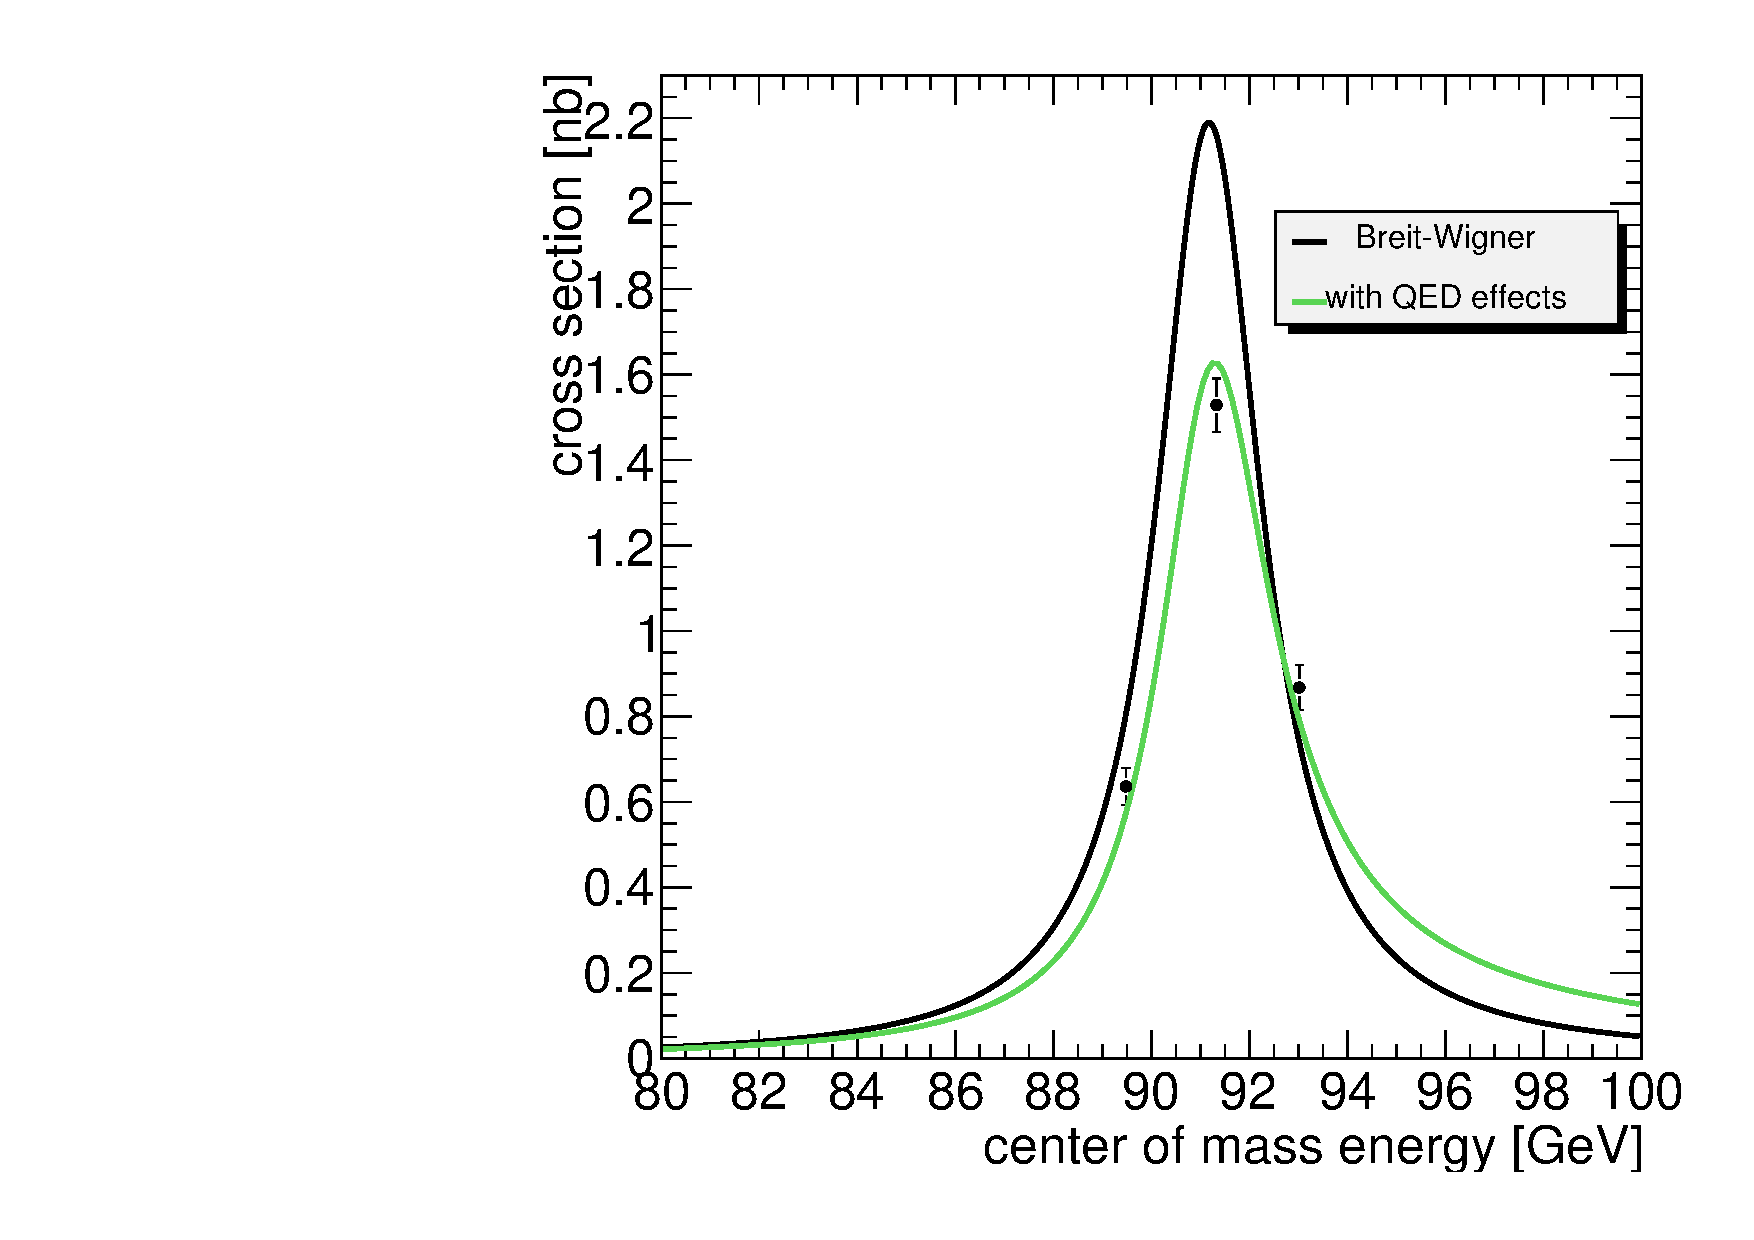
\includegraphics[width=1\columnwidth,keepaspectratio]{finalmu_fit}
 \caption{Breit-Wigner-Fit muons}
 \label{fig:n_cluster}
\end{figure}

\end{document}
